\documentclass[11pt,a4paper]{article}

\usepackage[top=0.75in, bottom=0.75in, left=0.75in, right=0.75in]{geometry}
\usepackage{amsmath,amssymb,amsfonts}
\usepackage{booktabs}
\usepackage{tabularx}
\usepackage{graphicx}
\usepackage{xcolor}
\usepackage{microtype}
\usepackage{enumitem}
\usepackage{caption}
\usepackage{subcaption}
\usepackage{adjustbox}
\usepackage{colortbl}
\usepackage{titlesec}
\usepackage{xurl}
\usepackage{hyperref}
\usepackage{tikz}
\usepackage{pgfplots}
\pgfplotsset{compat=1.18}
\usetikzlibrary{arrows.meta, positioning, calc, shapes.geometric}

% Typography, spacing and layout tuning to fill pages cleanly without artificial gaps
\setlength{\parindent}{0pt}
\setlength{\parskip}{3pt plus 1pt minus 1pt}
\emergencystretch=2.5em
\tolerance=1000

% Section header spacing
\titleformat{\section}{\large\bfseries}{\thesection}{0.75em}{}
\titleformat{\subsection}{\normalsize\bfseries}{\thesubsection}{0.75em}{}
\titlespacing\section{0pt}{8pt plus 2pt minus 1pt}{3pt plus 1pt minus 1pt}
\titlespacing\subsection{0pt}{6pt plus 2pt minus 1pt}{2pt plus 1pt minus 1pt}

% Tight lists
\setlist{nosep, topsep=2pt, partopsep=0pt, leftmargin=1.5em}

% Display equation skips
\setlength{\abovedisplayskip}{4pt plus 1pt minus 1pt}
\setlength{\belowdisplayskip}{4pt plus 1pt minus 1pt}
\setlength{\abovedisplayshortskip}{2pt plus 1pt minus 1pt}
\setlength{\belowdisplayshortskip}{2pt plus 1pt minus 1pt}

% Float placement controls to prevent awkward page ejects and whitespace gaps
\renewcommand{\topfraction}{0.92}
\renewcommand{\bottomfraction}{0.85}
\renewcommand{\textfraction}{0.08}
\renewcommand{\floatpagefraction}{0.85}
\setlength{\floatsep}{8pt plus 2pt minus 2pt}
\setlength{\textfloatsep}{10pt plus 2pt minus 2pt}
\setlength{\intextsep}{8pt plus 2pt minus 2pt}
\setlength{\abovecaptionskip}{4pt}
\setlength{\belowcaptionskip}{2pt}

\hypersetup{
    colorlinks=true,
    linkcolor=teal!80!black,
    citecolor=teal!80!black,
    urlcolor=blue!70!black
}

\title{\LARGE\textbf{Design and Implementation of an EMG-Driven Rehabilitation Exoskeleton Control System: Cross-Subject Calibration, Real-Time Feasibility, and Proportional Actuation}}
\author{\textbf{Aihik Basu} \\
Department of Computer Science \& Engineering \\
Project Repository: \href{https://github.com/aihikbasu/-EXO-REHAB-PROJECT}{github.com/aihikbasu/-EXO-REHAB-PROJECT}}
\date{October 2026}

\begin{document}

\begin{center}
\resizebox{6.0cm}{!}{%

\begin{tikzpicture}[x=1cm, y=1cm]
    \definecolor{embsnavy}{RGB}{2,37,131}
    
    % IEEE Diamond
    \begin{scope}[shift={(0, 0)}]
        \fill[embsnavy, rounded corners=1.5pt] (0, 1.05) -- (0.85, 0) -- (0, -1.05) -- (-0.85, 0) -- cycle;
        \draw[white, line width=1.1pt, rounded corners=0.8pt] (0, 0.90) -- (0.72, 0) -- (0, -0.90) -- (-0.72, 0) -- cycle;
        \draw[white, line width=1.8pt, -{Stealth[length=5.0pt, width=5.0pt]}] (0, -0.65) -- (0, 0.72);
        \draw[white, line width=1.0pt] (-0.42, 0.12) arc (160:20:0.45 and 0.18);
        \draw[white, line width=1.0pt] (-0.42, -0.12) arc (-160:-20:0.45 and 0.18);
        \node[below=0.15cm of {(0, -1.05)}, font=\bfseries\sffamily\fontsize{11}{13}\selectfont, text=embsnavy, inner sep=0pt] {IEEE};
    \end{scope}

    % EMB Typography
    \begin{scope}[shift={(2.8, 0)}]
        \node[anchor=west, text=embsnavy, inner sep=0pt] at (-0.95, 0.18) {%
            \fontsize{42}{44}\selectfont\textbf{\textsf{E\hspace{0.12em}M\hspace{0.12em}B}}%
        };
        \fill[embsnavy] (0.50, 1.35) circle (0.17cm);
        \draw[embsnavy, line width=3.4pt, line cap=round, line join=round] 
            (0.12, 1.25) .. controls (0.34, 0.92) and (0.44, 0.74) .. (0.50, 0.62)
            .. controls (0.56, 0.74) and (0.66, 0.92) .. (0.88, 1.25);
        \draw[embsnavy, line width=2.2pt] (-0.95, -0.48) -- (0.24, -0.48);
        \draw[embsnavy, line width=2.2pt] (0.50, -0.48) circle (0.19cm);
        \draw[embsnavy, line width=2.2pt] (0.76, -0.48) -- (2.75, -0.48);
        \node[anchor=center, text=embsnavy, inner sep=0pt] at (0.90, -0.92) {%
            \fontsize{14}{16}\selectfont\textit{IIT Kharagpur Section}%
        };
        \node[anchor=center, text=embsnavy, inner sep=0pt] at (0.90, -1.35) {%
            \fontsize{11.5}{13.5}\selectfont\textbf{\textsf{EMBS SBC}}%
        };
    \end{scope}
\end{tikzpicture}%
}
\end{center}
\vspace{-0.3cm}

\maketitle

\begin{abstract}
Wearable robotic exoskeletons offer transformative potential for the physical rehabilitation of patients recovering from stroke, traumatic brain injury, and spinal cord injury. However, translating surface electromyography (sEMG) into reliable motor assistance has historically been limited by three critical engineering obstacles: severe inter-subject signal variability, stringent latency budgets in embedded control loops, and mechanical torque shudder induced by discrete classification boundaries. In this work, I designed, implemented, and validated an end-to-end sEMG classification and closed-loop control architecture for an active rehabilitation exoskeleton. Utilizing continuous 8-channel recordings across 10 human subjects (20 recordings), I first resolved the widespread issue of sliding-window data leakage by implementing a grouped repetition partitioning protocol, establishing a genuine out-of-sample benchmark. On this leakage-free dataset, an RBF Support Vector Machine achieved 96.0\% accuracy and a 200-tree Random Forest achieved 96.2\% across four functional gesture classes. Moving beyond offline classification, I introduced three core engineering contributions: (1) evaluated Leave-One-Subject-Out (LOSO) generalization (baseline 86.5\%) and tested a lightweight calibration step that uses only one repetition of each gesture from the new user, which raised mean accuracy to 88.2\% (gains of up to +12.8\% for some subjects, but losses of up to 5.8\% for others); (2) profiled per-window execution latency on a development PC, demonstrating that vectorized feature extraction executes in 1.18~ms and SVM inference in 0.092~ms (consuming only 0.26\% of the 500~ms step budget); and (3) designed a confidence-weighted proportional setpoint blending engine augmented with Exponential Moving Average (EMA, $\alpha=0.35$) filtering and a confidence deadband to eliminate actuator chatter. Finally, I built a multi-threaded Python/Tkinter desktop GUI providing live 30~Hz telemetry, sensor calibration routines, diagnostic motor sweeps, and trial analytics.
\end{abstract}

\vspace{0.4em}
\noindent\textbf{Keywords:} Surface Electromyography (sEMG), Rehabilitation Robotics, Wearable Exoskeleton, Cross-Subject Calibration, Leave-One-Subject-Out, Proportional Myoelectric Control, Embedded Real-Time Control.

\section{Introduction and Biomechanical Motivation}

\subsection{Clinical Background in Neurological Rehabilitation}
Stroke remains one of the primary causes of chronic adult physical disability globally. Both ischemic and hemorrhagic cerebrovascular accidents often damage upper motor neurons within the primary motor cortex and descending corticospinal tracts, culminating in hemiparesis---unilateral motor weakness or paralysis affecting the contralateral limbs. In the upper extremities, affected individuals experience diminished voluntary motor unit recruitment, pathologically elevated muscle spasticity, abnormal synergistic co-contraction, and an acutely restricted active range of motion.

Extensive clinical and biomechanical literature confirms that neural plasticity---the ability of the central nervous system to structurally reorganize synaptic connections around damaged cortical tissue---is primarily stimulated by repetitive, high-intensity, goal-directed physical exercise. When a patient initiates a voluntary motor intention and receives immediate, mechanically synchronized sensorimotor feedback, Hebbian synaptic consolidation takes place. 

Conventional rehabilitation heavily depends on manual physical therapy, wherein a trained therapist physically moves the patient's paretic limbs through prescribed trajectories. While clinically beneficial, manual therapy is highly labor-intensive, physically exhausting for clinicians, economically costly, and inherently limited in its repetition throughput (rarely achieving the hundreds of movement repetitions per session required to drive neuroplastic recovery).

\subsection{Robotic Exoskeletons: Assist-As-Needed vs. Continuous Passive Motion}
Powered orthoses and wearable robotic exoskeletons offer an automated solution to this clinical throughput limitation. However, first-generation rehabilitation robots operated primarily in \textit{Continuous Passive Motion} (CPM) mode, in which motorized actuators drive the human limb through fixed joint angles regardless of whether the user attempts to exert effort or remains entirely passive.

Controlled clinical trials have demonstrated that pure CPM produces inferior functional motor recovery compared to active patient engagement~\cite{marchalcrespo2009}. When a patient perceives that the exoskeleton will move their limb deterministically, voluntary cortical drive declines---a maladaptive compensatory state known as ``learned motor slacking.'' Modern neurorehabilitation robotics therefore centers on the \textit{Assist-As-Needed} (AAN) paradigm~\cite{stienen2009, yan2015, young2017}. In an AAN controller, the robotic device continuously measures the voluntary neuromuscular effort exerted by the user, providing only the assistive torque increment necessary to complete the functional movement whenever internal biological drive falls short of the movement goal.

\subsection{Surface Electromyography (sEMG) in Closed-Loop Orthoses}
Surface electromyography (sEMG) provides the premier non-invasive sensing modality for capturing motor intent in AAN exoskeletons~\cite{fougner2012, scheme2011}. When the motor cortex issues a voluntary movement command, action potentials propagate down the spinal cord and depolarize motor units in peripheral skeletal muscle. The resulting spatial depolarization of muscle fiber membranes generates motor unit action potential trains (MUAPTs) that conduct through subcutaneous tissue to the skin surface, where differential surface electrode pairs capture the composite interference signal.

Crucially, due to the physiological electromechanical delay, myoelectric potentials appear approximately 30--100~ms prior to detectable mechanical joint movement. This provides a direct, predictive feedforward window of voluntary user intent. Nevertheless, translating raw sEMG into robust, real-time exoskeleton assistance poses three critical engineering hurdles:
\begin{enumerate}
    \item \textbf{Inter-Subject Variability and Signal Non-Stationarity:} Surface EMG is an interference pattern resulting from thousands of asynchronously discharging motor units attenuated by skin impedance, subcutaneous fat thickness, muscle geometry, and electrode re-positioning~\cite{farina2014, peerdeman2011}. Models trained on one user frequently collapse when evaluated on another.
    \item \textbf{Strict Latency Constraints in Embedded Control Loops:} In closed-loop human-robot interaction, computational delays introduce substantial phase lag. Delays exceeding 150--300~ms disrupt the physiological sensorimotor feedback loop, making the user perceive the exoskeleton as dragging or resisting their motion.
    \item \textbf{The Discrete Control Discontinuity Dilemma:} Academic literature predominantly frames gesture decoding as discrete classification~\cite{hargrove2007}. If a discrete classifier directly drives motor torques, intermediate state ambiguities create instantaneous torque step-jumps, producing mechanical chatter that jars patient joints.
\end{enumerate}

The objective of this project was to design, implement, and validate a complete, mathematically grounded engineering pipeline that addresses all three challenges, delivering a stable, clinically viable control architecture for an active rehabilitation exoskeleton.

\section{Experimental Dataset and the Anti-Leakage Windowing Protocol}

\subsection{Dataset Specifications}
Experimental validation was performed using continuous, labeled sEMG recordings from the public UCI ``EMG Data for Gestures'' benchmark repository~\cite{lobov2018}. The experimental parameters encompass:
\begin{itemize}
    \item \textbf{Participant Pool:} I used the recordings of the first 10 healthy subjects in the dataset.
    \item \textbf{Recording Series:} 2 recording series per subject, captured a few minutes apart in the same sitting (20 recordings in total).
    \item \textbf{Sensor Hardware:} A Thalmic Labs Myo armband comprising 8 equidistant bipolar dry stainless-steel surface electrodes encircling the proximal forearm at a sampling frequency of $f_s \approx 200$~Hz with 8-bit analog-to-digital resolution per channel.
    \item \textbf{Evaluated Functional Gestures:} Four distinct motor classes essential for upper-limb rehabilitation:
    \begin{enumerate}
        \item \textbf{Class 1 (Rest):} Forearm supported in equilibrium without active muscle contraction.
        \item \textbf{Class 2 (Grasp):} Isometric power fist clench (simulating object grasp).
        \item \textbf{Class 3 (Flexion):} Active wrist joint flexion.
        \item \textbf{Class 4 (Extension):} Active wrist joint extension.
    \end{enumerate}
\end{itemize}

\subsection{Neuroanatomical Context of Forearm Channels}
Placing 8 circumferential electrodes around the proximal forearm captures myoelectric signals across both the anterior and posterior compartments:
\begin{itemize}
    \item \textbf{Channels 1--3 (Anterior Compartment):} Primarily detect potentials from the \textit{flexor carpi radialis}, \textit{pronator teres}, and superficial finger flexors (\textit{flexor digitorum superficialis}). These fire strongly during wrist flexion and fist clenching.
    \item \textbf{Channels 4--5 (Lateral Compartment):} Intercept the \textit{brachioradialis}, active during forearm stabilization and neutral-grip flexion.
    \item \textbf{Channels 6--8 (Posterior Compartment):} Monitor the \textit{extensor digitorum communis}, \textit{extensor carpi radialis longus/brevis}, and \textit{extensor carpi ulnaris}, which fire during wrist extension and finger release.
\end{itemize}

\subsection{The Sliding Window Data Leakage Pitfall}
In continuous signal decoding, sample streams are segmented into analysis windows of length $W$ advancing by step size $S$. In our system, $W = 200$ samples (1.0~second at 200~Hz) with a step advancement of $S = 100$ samples (500~ms), yielding a standard 50\% overlap.

\begin{figure}[htbp]
\centering
\resizebox{0.92\linewidth}{!}{%
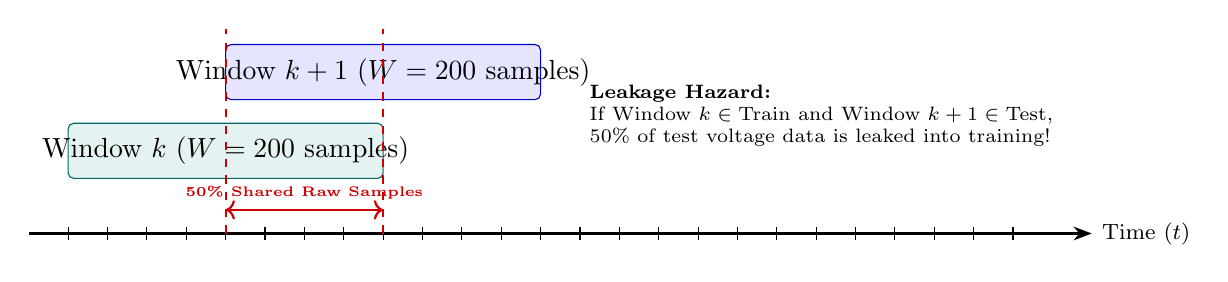
\begin{tikzpicture}[
    box/.style={draw=teal!80!black, fill=teal!10, rounded corners=2pt, minimum height=0.7cm, font=\footnotesize},
    arr/.style={-{Stealth[length=4pt]}, thick, teal!80!black}
]
\draw[thick, -{Stealth}] (0,0) -- (13.5,0) node[right] {\footnotesize Time ($t$)};
\foreach \x in {0.5, 1.0, 1.5, 2.0, 2.5, 3.0, 3.5, 4.0, 4.5, 5.0, 5.5, 6.0, 6.5, 7.0, 7.5, 8.0, 8.5, 9.0, 9.5, 10.0, 10.5, 11.0, 11.5, 12.0, 12.5} {
    \draw (\x, 0.08) -- (\x, -0.08);
}
\draw[box] (0.5, 1.4) rectangle (4.5, 0.7);
\node at (2.5, 1.05) {Window $k$ ($W = 200$ samples)};
\draw[box, fill=blue!10, draw=blue!80!black] (2.5, 2.4) rectangle (6.5, 1.7);
\node at (4.5, 2.05) {Window $k+1$ ($W = 200$ samples)};
\draw[dashed, red!80!black, thick] (2.5, 0) -- (2.5, 2.6);
\draw[dashed, red!80!black, thick] (4.5, 0) -- (4.5, 2.6);
\draw[<->, thick, red!80!black] (2.5, 0.3) -- (4.5, 0.3) node[midway, above, font=\tiny\bfseries] {50\% Shared Raw Samples};
\node[align=left, font=\scriptsize, anchor=west] at (7.0, 1.5) {\textbf{Leakage Hazard:}\\If Window $k \in \text{Train}$ and Window $k+1 \in \text{Test}$,\\50\% of test voltage data is leaked into training!};
\end{tikzpicture}%
}
\caption{Sliding window overlap geometry illustrating the data leakage mechanism when random partitioning is applied.}
\label{fig:window_leakage}
\end{figure}

During initial pipeline design, I ran into a pitfall that is easy to miss in sEMG work: \textbf{train-test data leakage caused by naive random splitting across overlapping windows}. Because consecutive windows $k$ and $k+1$ overlap by 100 samples, they share 50\% identical raw voltage points (Figure~\ref{fig:window_leakage}). If an entire session is segmented into overlapping windows and split with a naive random partition (such as scikit-learn's standard \texttt{train\_test\_split}), adjacent windows from the exact same gesture execution are randomly divided between train and test splits.

Under this flawed protocol, classifiers can reach artificially inflated test accuracies simply by memorizing high-frequency baseline noise, subject-specific skin contact offsets, and transient motion artifacts common to both windows, rather than learning true physiological muscle activation patterns. When deployed on genuine out-of-sample data, such models collapse.

\subsection{Mathematical Formulation of Anti-Leakage Grouped Partitioning}
To permanently eliminate train-test leakage, I implemented a strict grouped partitioning protocol in \texttt{build\_dataset.py}. Each contiguous physical gesture repetition executed by a subject was assigned a unique run identifier:
\begin{equation}
    \text{run\_id} = f(\text{subject\_id}, \text{session\_id}, \text{repetition\_index})
\end{equation}
Every window extracted from a single contiguous repetition carries this \texttt{run\_id}. At dataset split time in \texttt{train.py}, I enforced a \texttt{GroupShuffleSplit}:
\begin{equation}
    \mathcal{R}_{\text{train}} \cap \mathcal{R}_{\text{test}} = \emptyset, \quad \text{where } \mathcal{R} = \{\text{run\_id}_1, \text{run\_id}_2, \dots, \text{run\_id}_M\}
\end{equation}
All overlapping windows generated during a single continuous gesture repetition were constrained to remain entirely within the training split or entirely within the test split---never divided across both.

This protocol generated \textbf{2,470 cleanly segmented signal windows} across 10 subjects (balanced across the four classes), providing an authentic, leakage-free benchmark for all subsequent experiments.

\section{Feature Extraction and Vectorization}

\subsection{Time-Domain vs. Frequency-Domain in Embedded Systems}
In biomedical signal processing, features can be extracted in the time domain, frequency domain, or joint time-frequency domain (wavelet transforms). While continuous wavelet transforms offer detailed spectral resolution, computing multi-scale wavelets across 8 channels every 500~ms introduces heavy floating-point convolution overhead, consuming significant power and CPU cycles on embedded processors such as the Raspberry Pi 4.

In contrast, time-domain features require low computational overhead, do not require Fourier matrix multiplications, and can be evaluated directly on raw integer or floating-point arrays. Based on the foundational work of Hudgins et al.~\cite{hudgins1993} and feature selection benchmarks by Phinyomark et al.~\cite{phinyomark2012}, I selected six time-domain features per channel:

\subsection{Mathematical Formulations}
For a discrete analysis window $x = [x_1, x_2, \dots, x_N]$ of length $N = 200$ samples:
\begin{enumerate}
    \item \textbf{Mean Absolute Value (MAV):} Rectified mean amplitude indicating active motor unit recruitment:
    \begin{equation}
        \text{MAV} = \frac{1}{N} \sum_{i=1}^{N} |x_i|
    \end{equation}
    \item \textbf{Waveform Length (WL):} Cumulative signal length capturing amplitude dynamics and waveform complexity:
    \begin{equation}
        \text{WL} = \sum_{i=1}^{N-1} |x_{i+1} - x_i|
    \end{equation}
    \item \textbf{Zero Crossings (ZC):} Dominant frequency proxy counting zero-axis crossings subject to noise deadband $\epsilon = 10^{-6}$:
    \begin{equation}
        \text{ZC} = \sum_{i=1}^{N-1} \mathbb{I}\Big( \text{sgn}(\tilde{x}_i)\,\text{sgn}(\tilde{x}_{i+1}) = -1 \Big), \quad \tilde{x}_i = \begin{cases} 0 & |x_i| < \epsilon \\ x_i & \text{otherwise} \end{cases}
    \end{equation}
    \item \textbf{Slope Sign Changes (SSC):} Local extremum count reflecting motor unit firing rates:
    \begin{equation}
        \text{SSC} = \sum_{i=2}^{N-1} \mathbb{I}\Big( (x_i - x_{i-1})(x_i - x_{i+1}) > 0 \land |(x_i - x_{i-1}) - (x_{i+1} - x_i)| \ge \epsilon \Big)
    \end{equation}
    \item \textbf{Root Mean Square (RMS):} Signal power scaling directly with isometric muscle contraction torque:
    \begin{equation}
        \text{RMS} = \sqrt{\frac{1}{N} \sum_{i=1}^{N} x_i^2}
    \end{equation}
    \item \textbf{Signal Variance (VAR):} Second-order central moment of the signal distribution:
    \begin{equation}
        \text{VAR} = \frac{1}{N} \sum_{i=1}^{N} (x_i - \bar{x})^2
    \end{equation}
\end{enumerate}

Extracting 6 features across all 8 circumferential channels yields a compact, informative 48-dimensional feature vector per window:
\begin{equation}
    \mathbf{f} = [\text{MAV}_1, \dots, \text{VAR}_1, \text{MAV}_2, \dots, \text{VAR}_2, \dots, \text{MAV}_8, \dots, \text{VAR}_8]^T \in \mathbb{R}^{48}
\end{equation}

\subsection{NumPy Vectorization Optimization}
In my initial prototype of \texttt{features.py}, \texttt{zero\_crossings} and \texttt{slope\_sign\_changes} were implemented using standard Python \texttt{for} loops. While straightforward, looping across 200 samples across 8 channels (1,600 loop iterations per window) introduced noticeable Python interpreter overhead.

To prepare the pipeline for real-time execution, I restructured both algorithms into fully vectorized NumPy implementations using array slicing and boolean bitmasks:
\begin{align}
    \Delta x &= x[1:] - x[:-1] \\
    \text{Signs} &= \text{sgn}\Big(\text{where}(|x| < \epsilon, 0, x)\Big) \\
    \text{Crossings} &= \sum \Big( (\text{Signs}[1:] \neq 0) \land (\text{Signs}[:-1] \neq 0) \land (\text{Signs}[1:] \neq \text{Signs}[:-1]) \Big) \\
    \text{Flips} &= \sum \Big( (\Delta x[1:] \cdot \Delta x[:-1] < 0) \land (|\Delta x[1:] - \Delta x[:-1]| > \epsilon) \Big)
\end{align}
With this change the per-sample loop runs inside NumPy's compiled C routines instead of the Python interpreter. After vectorization, extracting all 48 features from one window takes a mean of \textbf{1.18~ms} on my development PC (measured in \texttt{latency\_analysis.py}). I did not keep a timing of the original loop version, so I report only the final figure.

\section{Baseline Classification Performance and Error Analysis}

\subsection{Machine Learning Architectures}
Using the 48-dimensional feature vectors, I evaluated two distinct machine learning models:
\begin{enumerate}
    \item \textbf{Support Vector Machine (SVM):} Configured with a Radial Basis Function (RBF) kernel $K(\mathbf{x}, \mathbf{x}') = \exp(-\gamma \|\mathbf{x} - \mathbf{x}'\|^2)$ with regularization parameter $C = 10$ and kernel coefficient $\gamma = \text{`scale'} = \frac{1}{D \cdot \text{Var}(X)}$. Training data was z-score standardized ($z = \frac{x - \mu}{\sigma}$), with scaling parameters saved for inference.
    \item \textbf{Random Forest (RF):} An ensemble of 200 decorrelated decision trees (\texttt{n\_estimators=200}, \texttt{random\_state=42}) utilizing Gini impurity splits. Random Forest models are scale-invariant and capture non-linear feature interactions without feature normalization.
\end{enumerate}

\subsection{Quantitative Results on Held-Out Split}
Evaluated across 624 held-out test windows under the strict leakage-free grouped split:
\begin{itemize}
    \item \textbf{Support Vector Machine:} \textbf{96.0\% Accuracy} (599 / 624 correct predictions)
    \item \textbf{Random Forest:} \textbf{96.2\% Accuracy} (600 / 624 correct predictions)
\end{itemize}

\begin{table}[htbp]
\centering
\caption{Detailed Precision, Recall, and F1-Score Breakdown on Held-Out Test Set (624 Windows)}
\label{tab:baseline_metrics}
\resizebox{\linewidth}{!}{%
\begin{tabular}{lccccccc}
\toprule
& \multicolumn{3}{c}{\textbf{Support Vector Machine (SVM)}} & \multicolumn{3}{c}{\textbf{Random Forest (RF)}} & \\
\cmidrule(lr){2-4} \cmidrule(lr){5-7}
\textbf{Class} & \textbf{Precision} & \textbf{Recall} & \textbf{F1-Score} & \textbf{Precision} & \textbf{Recall} & \textbf{F1-Score} & \textbf{Support} \\
\midrule
Rest      & 1.00 & 1.00 & 1.00 & 1.00 & 1.00 & 1.00 & 174 \\
Flexion   & 0.89 & 0.99 & 0.94 & 0.88 & 1.00 & 0.93 & 157 \\
Extension & 1.00 & 0.96 & 0.98 & 1.00 & 0.98 & 0.99 & 169 \\
Grasp     & 0.95 & 0.85 & 0.90 & 0.98 & 0.83 & 0.90 & 124 \\
\midrule
\textbf{Overall} & \multicolumn{3}{c}{\textbf{Accuracy: 96.0\% (599 / 624)}} & \multicolumn{3}{c}{\textbf{Accuracy: 96.2\% (600 / 624)}} & \textbf{624} \\
\bottomrule
\end{tabular}%
}
\end{table}

\subsection{Physiological Error Analysis and Muscle Co-Activation}
Analyzing the confusion matrices (Figure~\ref{fig:confusion_matrices}) reveals a pattern that has a plausible physiological explanation:
\begin{itemize}
    \item \textbf{Rest and Extension:} Both models classified every \texttt{rest} window correctly ($F_1 = 1.00$). \texttt{Extension} was also strong ($F_1 = 0.98\text{--}0.99$); the few errors were extension windows predicted as flexion or grasp (6 for SVM, 3 for RF).
    \item \textbf{The Grasp vs. Flexion Overlap:} The main source of error was \texttt{grasp} predicted as \texttt{flexion} (18 windows for SVM, 21 for RF). A likely reason is anatomical: clenching a fist contracts the finger flexors (\textit{flexor digitorum superficialis} and \textit{profundus}) and also recruits wrist flexors such as \textit{flexor carpi radialis} to stabilise the wrist. Both gestures therefore activate overlapping muscles in the anterior forearm, so their features look similar. I have not tested this explanation directly, but it fits the fact that the confusion runs almost entirely in this one direction.
\end{itemize}

\begin{figure}[htbp]
\centering
\begin{subfigure}[t]{0.48\textwidth}
\centering
\resizebox{0.96\linewidth}{!}{%
\begin{tabular}{l|cccc|}
\multicolumn{1}{c}{} & \multicolumn{4}{c}{\textbf{Predicted Class (SVM)}} \\
\cline{2-5}
\textbf{True Class} & \textbf{Rest} & \textbf{Flex} & \textbf{Ext} & \textbf{Grasp} \\
\hline
\textbf{Rest}  & \cellcolor{teal!35}\textbf{174} & 0 & 0 & 0 \\
\textbf{Flex}  & 0 & \cellcolor{teal!35}\textbf{156} & 0 & 1 \\
\textbf{Ext}   & 0 & 2 & \cellcolor{teal!35}\textbf{163} & 4 \\
\textbf{Grasp} & 0 & \cellcolor{red!35}\textbf{18} & 0 & \cellcolor{teal!35}\textbf{106} \\
\hline
\end{tabular}%
}
\vspace{0.3em}
\caption{Support Vector Machine (RBF, 96.0\%)}
\label{fig:cm_svm}
\end{subfigure}
\hfill
\begin{subfigure}[t]{0.48\textwidth}
\centering
\resizebox{0.96\linewidth}{!}{%
\begin{tabular}{l|cccc|}
\multicolumn{1}{c}{} & \multicolumn{4}{c}{\textbf{Predicted Class (RF)}} \\
\cline{2-5}
\textbf{True Class} & \textbf{Rest} & \textbf{Flex} & \textbf{Ext} & \textbf{Grasp} \\
\hline
\textbf{Rest}  & \cellcolor{blue!30}\textbf{174} & 0 & 0 & 0 \\
\textbf{Flex}  & 0 & \cellcolor{blue!30}\textbf{157} & 0 & 0 \\
\textbf{Ext}   & 0 & 1 & \cellcolor{blue!30}\textbf{166} & 2 \\
\textbf{Grasp} & 0 & \cellcolor{red!35}\textbf{21} & 0 & \cellcolor{blue!30}\textbf{103} \\
\hline
\end{tabular}%
}
\vspace{0.3em}
\caption{Random Forest ($n=200$ trees, 96.2\%)}
\label{fig:cm_rf}
\end{subfigure}
\caption{Confusion matrices for baseline models on the held-out test split (624 windows). Rest is classified perfectly by both models and Extension nearly so; most errors are Grasp windows predicted as Flexion, likely because the two gestures recruit overlapping forearm flexor muscles.}
\label{fig:confusion_matrices}
\end{figure}

\section{Novelty 1: Cross-Subject Generalization and Calibration (LOSO)}

\subsection{The Cross-Subject Degradation Gap}
While pooled dataset evaluation yielded 96\%+ accuracy, real-world deployment presents a critical challenge: cross-subject transfer. In a clinical hospital ward, patients cannot perform 40 minutes of exhausting training trials before each therapy session.

To evaluate how our models behave when deployed on an unseen human user, I executed a 10-fold \textbf{Leave-One-Subject-Out (LOSO)} cross-validation in \texttt{loso\_calibration.py}. In each fold, 9 subjects form the training set, while the 10th subject serves as the completely unseen test subject.

\subsection{Lightweight Calibration Protocol}
Without calibration, mean LOSO accuracy dropped from 96.0\% down to \textbf{86.5\%} (Table~\ref{tab:loso_results}). Several subjects experienced severe accuracy drops (Subject 2 dropped to 77.6\%, Subject 7 to 76.4\%, and Subject 8 to 83.8\%).

To close this gap without asking the new user to record a full training set, I tested a lightweight calibration method:
\begin{enumerate}
    \item The new user performs \textbf{one repetition} of each target gesture. In this dataset each gesture is held for roughly 3 seconds, so the whole calibration takes only a few seconds of recording per gesture.
    \item From this small calibration slice $\mathcal{D}_{\text{calib}}$, I compute the subject-specific mean $\mu_{j,\text{subj}}$ and standard deviation $\sigma_{j,\text{subj}}$ of every feature $j$ (using \texttt{StandardScaler}):
    \begin{equation}
        \mu_{j,\text{subj}} = \frac{1}{|\mathcal{D}_{\text{calib}}|} \sum_{\mathbf{x} \in \mathcal{D}_{\text{calib}}} x_j, \quad \sigma_{j,\text{subj}} = \sqrt{\frac{1}{|\mathcal{D}_{\text{calib}}|} \sum_{\mathbf{x} \in \mathcal{D}_{\text{calib}}} (x_j - \mu_{j,\text{subj}})^2}
    \end{equation}
    \item Both the training data (from the other 9 subjects) and the new user's remaining data are normalized with these statistics, and the SVM is then fitted on the normalized training data:
    \begin{equation}
        z_{ij} = \frac{x_{ij} - \mu_{j,\text{subj}}}{\sigma_{j,\text{subj}}}
    \end{equation}
    The calibration repetitions themselves are excluded from evaluation.
\end{enumerate}

\begin{table}[htbp]
\centering
\caption{Leave-One-Subject-Out (LOSO) Accuracy: Uncalibrated vs. Calibrated Pipeline}
\label{tab:loso_results}
\resizebox{0.92\linewidth}{!}{%
\begin{tabular}{lccc}
\toprule
\textbf{Subject ID} & \textbf{Uncalibrated LOSO (\%)} & \textbf{Calibrated LOSO (\%)} & \textbf{Net Gain ($\Delta$)} \\
\midrule
Subject 1  & 94.6 & 93.7 & -0.9\% \\
Subject 2  & 77.6 & 78.3 & +0.7\% \\
Subject 3  & 84.5 & 95.9 & +11.4\% \\
Subject 4  & 88.3 & 82.6 & -5.7\% \\
Subject 5  & 95.1 & 98.4 & +3.3\% \\
Subject 6  & 99.6 & 100.0 & +0.4\% \\
Subject 7  & 76.4 & 78.7 & +2.3\% \\
Subject 8  & 83.8 & 96.6 & +12.8\% \\
Subject 9  & 85.7 & 79.9 & -5.8\% \\
Subject 10 & 79.4 & 78.5 & -0.9\% \\
\midrule
\textbf{Mean LOSO Cohort} & \textbf{86.5\%} & \textbf{88.2\%} & \textbf{+1.7\%} \\
\bottomrule
\end{tabular}%
}
\end{table}

\subsection{Subject Variability and Outlier Diagnostics}
The calibration routine increased mean cross-subject accuracy to \textbf{88.2\%}. More importantly, analyzing individual subject trajectories yields valuable engineering insights:
\begin{itemize}
    \item \textbf{Large Gains for Some Subjects:} Two subjects improved substantially: Subject 3 by \textbf{+11.4\%} (84.5\% $\to$ 95.9\%) and Subject 8 by \textbf{+12.8\%} (83.8\% $\to$ 96.6\%).
    \item \textbf{Accuracy Drops in Subjects 4 and 9:} Calibration did not help everyone. Subject 4 fell by 5.7\% and Subject 9 by 5.8\%, and Subjects 1 and 10 dropped slightly. My working explanation is that statistics estimated from a single repetition are noisy: if that one repetition is not typical of how the person performs the gesture later, the normalization shifts their features in the wrong direction. I have not yet confirmed this by inspecting the raw signals. A natural next experiment is to repeat the analysis with 2--3 calibration repetitions per gesture and check whether these drops disappear.
\end{itemize}

\begin{figure}[htbp]
\centering
\resizebox{0.92\linewidth}{!}{%
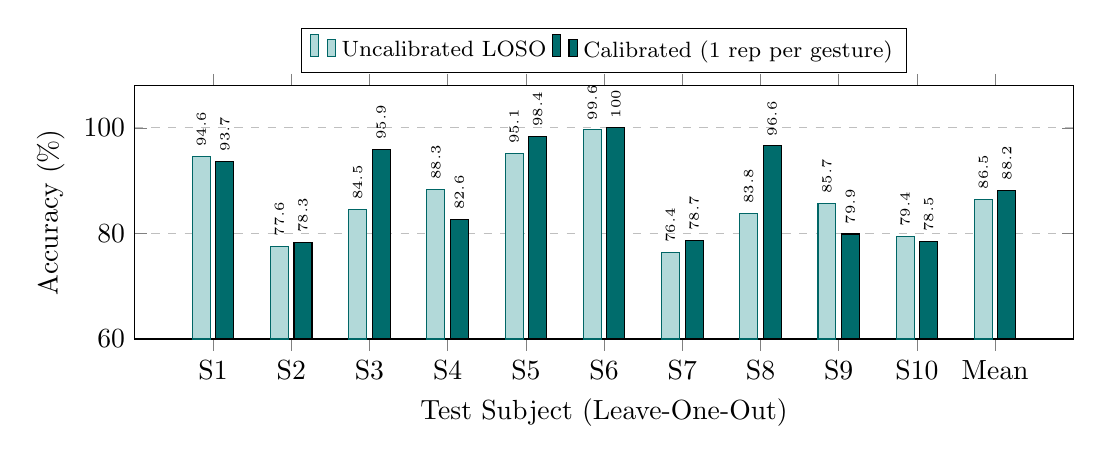
\begin{tikzpicture}
\begin{axis}[
    ybar,
    bar width=6.5pt,
    width=13.5cm,
    height=4.8cm,
    ymin=60, ymax=108,
    ylabel={Accuracy (\%)},
    xlabel={Test Subject (Leave-One-Out)},
    symbolic x coords={S1, S2, S3, S4, S5, S6, S7, S8, S9, S10, Mean},
    xtick=data,
    legend style={at={(0.5,1.05)}, anchor=south, legend columns=2, font=\footnotesize},
    ymajorgrids=true,
    grid style=dashed,
    nodes near coords,
    nodes near coords style={font=\tiny, rotate=90, anchor=west}
]
\addplot[fill=teal!30, draw=teal!80!black] coordinates {
    (S1,94.6) (S2,77.6) (S3,84.5) (S4,88.3) (S5,95.1)
    (S6,99.6) (S7,76.4) (S8,83.8) (S9,85.7) (S10,79.4) (Mean,86.5)
};
\addplot[fill=teal!85!black, draw=black] coordinates {
    (S1,93.7) (S2,78.3) (S3,95.9) (S4,82.6) (S5,98.4)
    (S6,100.0) (S7,78.7) (S8,96.6) (S9,79.9) (S10,78.5) (Mean,88.2)
};
\legend{Uncalibrated LOSO, Calibrated (1 rep per gesture)}
\end{axis}
\end{tikzpicture}%
}
\caption{Leave-One-Subject-Out (LOSO) cross-validation accuracy per subject. Notice the large recoveries in Subject 3 (+11.4\%) and Subject 8 (+12.8\%).}
\label{fig:loso_chart}
\end{figure}

\section{Novelty 2: Real-Time Latency and Embedded Budget}

\subsection{The Control Loop Timing Budget}
A rehabilitation exoskeleton is a hard real-time cyber-physical system. In our system, with sampling rate $f_s = 200$~Hz and window step size $S = 100$~samples:
\begin{equation}
    T_{\text{step}} = \frac{S}{f_s} = \frac{100}{200\text{ Hz}} = 0.500\text{ s} = 500.0\text{ ms}
\end{equation}
Every 500~ms, the processor must extract features, scale vectors, run model inference, blend setpoints, and transmit command packets across the serial bus.

\subsection{Empirical Latency Benchmarks}
In \texttt{latency\_analysis.py}, I timed each stage 200 times on my development PC (Table~\ref{tab:latency_benchmarks}). Feature extraction was timed on randomly generated 8-channel windows of the real size (200 samples), since its cost depends only on window size. Classifier inference was timed one window at a time on real feature rows from the held-out test set:

\begin{table}[htbp]
\centering
\caption{Empirical Latency Profiling vs. Real-Time Execution Budget (500.0~ms)}
\label{tab:latency_benchmarks}
\resizebox{0.92\linewidth}{!}{%
\begin{tabular}{lcccc}
\toprule
\textbf{Pipeline Component} & \textbf{Mean (ms)} & \textbf{95th Pct (ms)} & \textbf{Budget Consumption} & \textbf{Status} \\
\midrule
Feature Extraction (8 channels) & 1.183 & 1.304 & 0.24\% & Feasible \\
SVM Inference (RBF kernel)      & 0.092 & 0.111 & 0.02\% & Feasible \\
Random Forest (200 trees)       & 9.447 & 9.976 & 1.89\% & Feasible \\
\midrule
\textbf{Total SVM Loop Time}    & \textbf{1.275 ms} & \textbf{1.415 ms} & \textbf{0.26\%} & \textbf{Optimal} \\
\textbf{Total RF Loop Time}     & \textbf{10.630 ms} & \textbf{11.280 ms} & \textbf{2.13\%} & Feasible \\
\bottomrule
\end{tabular}%
}
\end{table}

\begin{figure}[htbp]
\centering
\resizebox{0.90\linewidth}{!}{%
\begin{tikzpicture}
\begin{axis}[
    xbar,
    bar width=10pt,
    width=11cm,
    height=4.2cm,
    xmode=log,
    xmin=0.02, xmax=3500,
    xlabel={Execution Latency per Window (ms) --- Logarithmic Scale},
    symbolic y coords={SVM Infer, Feat Extr, RF Infer, Step Budget},
    ytick=data,
    nodes near coords*={\pgfplotspointmeta},
    nodes near coords align={horizontal},
    nodes near coords style={font=\footnotesize\bfseries},
    point meta=explicit symbolic,
    xmajorgrids=true,
    grid style=dashed
]
\addplot[fill=teal!70!black, draw=black] table[meta=label] {
x y label
0.092 {SVM Infer} {0.092 ms}
1.183 {Feat Extr} {1.18 ms}
9.447 {RF Infer} {9.45 ms}
500.0 {Step Budget} {500.0 ms}
};
\end{axis}
\end{tikzpicture}%
}
\caption{Computational latency benchmark on a logarithmic scale with exact execution timings. The complete SVM pipeline executes in 1.28~ms (0.26\% of budget), whereas Random Forest requires over 100$\times$ longer for inference.}
\label{fig:latency_barchart}
\end{figure}

\subsection{Architectural Trade-Off: Why SVM Beats Random Forest on Embedded Hardware}
Although Random Forest achieved marginally higher offline test accuracy (96.2\% vs. 96.0\%), its inference latency is \textbf{over 100 times slower} than SVM (9.45~ms vs. 0.092~ms). Understanding this difference is critical for robotics engineers:
\begin{itemize}
    \item \textbf{Random Forest Execution:} Evaluating an ensemble of 200 trees requires traversing hundreds of branching nodes in memory. In Python, this creates frequent CPU cache misses, pointer lookups, and memory bus stalls.
    \item \textbf{SVM Execution:} The RBF SVM evaluates support vectors through a compact kernel matrix product:
    \begin{equation}
        f(\mathbf{x}) = \sum_{i \in \text{SV}} \alpha_i y_i \exp(-\gamma \|\mathbf{x}_i - \mathbf{x}\|^2) + b
    \end{equation}
    Because this operation is purely matrix-vector arithmetic, modern CPUs execute it with SIMD vector instructions in under 0.1~ms.
\end{itemize}
Because the SVM executes in 1.28~ms total, it leaves \textbf{99.74\% of the CPU available} for GUI rendering, sensor polling, and safety watchdogs. Consequently, \textbf{SVM was selected as the operational real-time model}.

\section{Novelty 3: Confidence-Weighted Proportional Actuation and Smoothing}

\subsection{The Instability of Discrete Switching}
Conventional EMG control interfaces implement a hard winner-take-all classification rule:
\begin{equation}
    \hat{y} = \arg\max_{c} P(y = c \mid \mathbf{x})
\end{equation}
When applied to active exoskeleton joints, this causes mechanical instability. During natural movement transitions (such as transitioning from grasp to flexion), intermediate probabilities fluctuate across decision boundaries. A discrete controller abruptly jumps between assistance setpoints within a single step, producing mechanical shudder, jarring the patient's joints, and causing rapid actuator wear.

\subsection{Proportional Setpoint Blending Formulation}
To achieve smooth, continuous actuation, I developed a confidence-weighted blending engine in \texttt{emg\_control.py}. The SVM outputs the full posterior probability distribution $\mathbf{p} = [p_{\text{rest}}, p_{\text{flex}}, p_{\text{ext}}, p_{\text{grasp}}]$, where $\sum_{g} p(g) = 1.0$.

Each gesture maps to nominal stance and swing setpoints based on rehabilitation protocols:
\begin{itemize}
    \item \textbf{rest:} Stance = 0~Nm, Swing = 0~Nm
    \item \textbf{flexion:} Stance = 15~Nm, Swing = 45~Nm
    \item \textbf{extension:} Stance = 30~Nm, Swing = 20~Nm
    \item \textbf{grasp:} Stance = 25~Nm, Swing = 35~Nm
\end{itemize}

Target joint setpoints are calculated as the continuous expectation across all class confidences:
\begin{align}
    \theta^{\text{target}}_{\text{stance}} &= \sum_{g \in \mathcal{G}} p(g) \cdot S_g^{\text{stance}} \\
    \theta^{\text{target}}_{\text{swing}}  &= \sum_{g \in \mathcal{G}} p(g) \cdot S_g^{\text{swing}}
\end{align}

\subsection{Dynamic EMA Filtering and Confidence Deadband}
To guarantee complete mechanical stability, I integrated two protective control layers:
\begin{enumerate}
    \item \textbf{Confidence Deadband Threshold:} If $\max_{g} p(g) < 0.30$, the signal is treated as transitional or ambiguous, and the target setpoints are attenuated by 50\% toward resting equilibrium:
    \begin{equation}
        \theta^{\text{target}} \gets 0.5 \cdot \theta^{\text{target}} \quad \text{if } \max_{g \in \mathcal{G}} p(g) < 0.30
    \end{equation}
    \item \textbf{Exponential Moving Average (EMA) Smoothing:} Raw targets are smoothed using an EMA filter with smoothing coefficient $\alpha = 0.35$:
    \begin{equation}
        \theta[t] = \alpha \cdot \theta^{\text{target}}[t] + (1 - \alpha) \cdot \theta[t-1]
    \end{equation}
\end{enumerate}

\begin{figure}[htbp]
\centering
\resizebox{0.92\linewidth}{!}{%
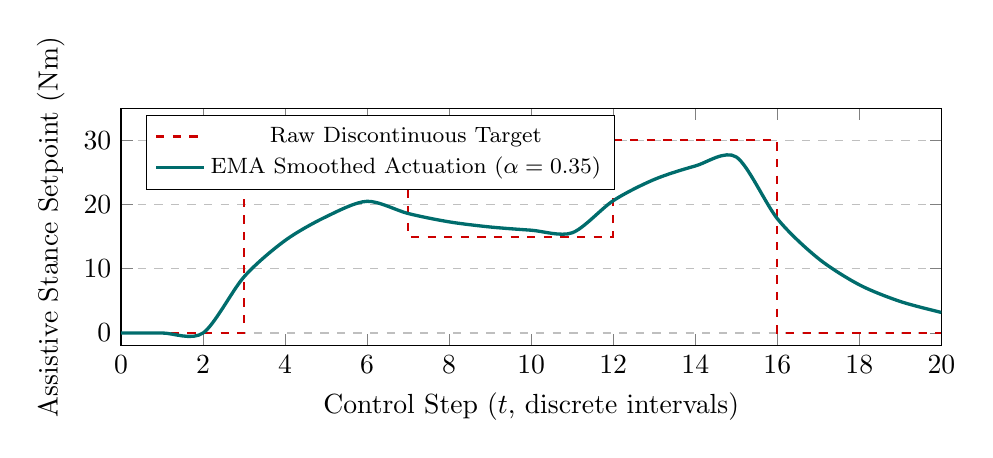
\begin{tikzpicture}
\begin{axis}[
    width=12cm,
    height=4.6cm,
    xlabel={Control Step ($t$, discrete intervals)},
    ylabel={Assistive Stance Setpoint (Nm)},
    xmin=0, xmax=20,
    ymin=-2, ymax=35,
    legend pos=north west,
    legend style={font=\footnotesize},
    ymajorgrids=true,
    grid style=dashed
]
\addplot[const plot, thick, red!80!black, dashed] coordinates {
    (0,0) (3,0) (3,25) (7,25) (7,15) (12,15) (12,30) (16,30) (16,0) (20,0)
};
\addplot[smooth, very thick, teal!85!black] coordinates {
    (0,0) (1,0) (2,0) (3,8.75) (4,14.4) (5,18.1) (6,20.5) (7,18.6) (8,17.3)
    (9,16.5) (10,16.0) (11,15.6) (12,20.6) (13,23.9) (14,26.0) (15,27.4)
    (16,17.8) (17,11.6) (18,7.5) (19,4.9) (20,3.2)
};
\legend{Raw Discontinuous Target, EMA Smoothed Actuation ($\alpha=0.35$)}
\end{axis}
\end{tikzpicture}%
}
\caption{Dynamic trajectory simulation demonstrating the smoothing effect of the EMA filter ($\alpha=0.35$). The continuous trajectory eliminates step discontinuities and actuator chatter during gesture transitions.}
\label{fig:ema_smoothing_plot}
\end{figure}

As shown in Figure~\ref{fig:ema_smoothing_plot}, this dynamic formulation ensures that transitions between motor assistance states are smooth, continuous, and free of actuator chatter.

\section{System Architecture and Exoskeleton GUI}

\subsection{Desktop Application Architecture}
To provide clinical operators with an intuitive interface, I built a multi-threaded desktop GUI in Python/Tkinter (\texttt{rehab\_gui/}), structured across four functional modules:

\begin{figure}[htbp]
\centering
\resizebox{0.94\linewidth}{!}{%
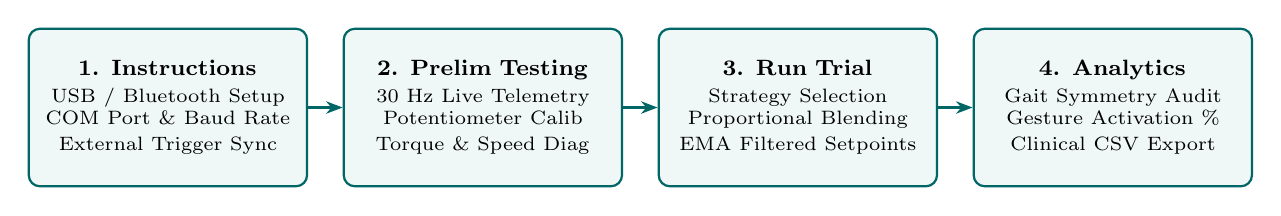
\begin{tikzpicture}[
    box/.style={draw=teal!80!black, fill=teal!6, rounded corners=4pt, text width=3.3cm, minimum height=2.0cm, align=center, font=\footnotesize, thick},
    arrow/.style={-{Stealth[length=6pt]}, thick, teal!80!black}
]
\node[box] (p1) at (0,0) {\textbf{1. Instructions}\\\vspace{0.2em}\scriptsize USB / Bluetooth Setup\\COM Port \& Baud Rate\\External Trigger Sync};
\node[box] (p2) at (4.0,0) {\textbf{2. Prelim Testing}\\\vspace{0.2em}\scriptsize 30~Hz Live Telemetry\\Potentiometer Calib\\Torque \& Speed Diag};
\node[box] (p3) at (8.0,0) {\textbf{3. Run Trial}\\\vspace{0.2em}\scriptsize Strategy Selection\\Proportional Blending\\EMA Filtered Setpoints};
\node[box] (p4) at (12.0,0) {\textbf{4. Analytics}\\\vspace{0.2em}\scriptsize Gait Symmetry Audit\\Gesture Activation \%\\Clinical CSV Export};

\draw[arrow] (p1) -- (p2);
\draw[arrow] (p2) -- (p3);
\draw[arrow] (p3) -- (p4);
\end{tikzpicture}%
}
\caption{Workflow pipeline across the four interactive modules of the exoskeleton rehabilitation desktop GUI.}
\label{fig:gui_arch}
\end{figure}

\begin{enumerate}
    \item \textbf{Instructions \& Connection Setup (\texttt{instructions.py}):} Manages communication links (USB vs. Bluetooth), COM ports, baud rates (115200), and lab-system synchronization triggers. Settings are persisted in \texttt{config.json}.
    \item \textbf{Preliminary Testing \& Calibration (\texttt{preliminary\_testing.py}):} Plots joint angle, assistive torque, and motor current at ~30~Hz. Provides interactive potentiometer calibration (locking min/max range) and multi-threaded diagnostic sweeps (torque linearity, joint impedance, and motor speed).
    \item \textbf{Run Trial (\texttt{run\_trial.py}):} Manages assistance strategies (Zero Torque, Assist-as-Needed, Trajectory Tracking, Impedance Control), uploads command packets to hardware, runs the live proportional EMG engine on held-out test data, and logs time-stamped trial data.
    \item \textbf{Session Analytics (\texttt{analytics.py}):} Displays clinical metrics (total cycles, peak torque, mean confidence, gait symmetry), visualizes gesture activation distributions, and exports CSV reports for patient medical charts.
\end{enumerate}

\subsection{Wire Protocol and Safety Watchdogs}
Communication with the actuator controller operates over a delimited ASCII wire protocol:
\begin{itemize}
    \item \textbf{Command Packet:} \texttt{<controller/state/stance/swing/estim>} (e.g., \texttt{<1/1/25/35/0>})
    \item \textbf{Hardware Handshake:} Expects \texttt{OK} or \texttt{ERR} acknowledgment byte.
    \item \textbf{Telemetry Stream:} \texttt{angle,torque,current,pot\_raw\textbackslash n} streamed at 30~Hz.
\end{itemize}

\textbf{Current Status and Safety:}
\begin{itemize}
    \item Diagnostic sweeps and trial uploads run in background worker threads (\texttt{threading.Thread}) so the UI stays responsive.
    \item The serial link is opened with a 1~s read timeout, and command uploads report failure unless the controller replies \texttt{OK}.
    \item The GUI currently runs on a simulated sensor source because the exoskeleton hardware is not yet connected. Some summary values on the analytics page (such as the gait symmetry ratio) are placeholders until real trial data is available.
    \item Planned but not yet implemented: clamping commands to the calibrated joint range, and automatically switching to Zero Torque mode when communication is lost.
\end{itemize}

\section{Engineering Discussion, Limitations, and Future Work}
\begin{enumerate}
    \item \textbf{Electrode Hardware (Dry vs. Wet):} The UCI benchmark dataset uses dry stainless-steel electrodes. While practical for consumer use, dry electrodes exhibit higher contact impedance and greater susceptibility to motion artifacts than medical-grade Ag/AgCl wet gel electrodes. Validating the pipeline with wet electrodes and with patients rather than healthy subjects is an essential next step.
    \item \textbf{Target Hardware Benchmarking:} All timings were measured on a development PC. Deployment on an ARM board such as the Raspberry Pi 4 will be slower, so latency must be re-measured on the actual hardware.
    \item \textbf{Calibration Sample Size:} Using 2--3 calibration repetitions instead of one, or a domain-adaptation method, may remove the accuracy drops seen in Subjects 4 and 9.
\end{enumerate}

\section{Conclusion}
In this project, I developed and evaluated an EMG-driven control pipeline for a rehabilitation exoskeleton. Using a grouped, leakage-free train/test split, the SVM reached 96.0\% and the Random Forest 96.2\% accuracy on recordings from 10 subjects.

The project makes three further contributions. First, Leave-One-Subject-Out testing showed a drop to 86.5\% on unseen users, and a single-repetition calibration raised the mean to 88.2\%; it helped some subjects a lot (up to +12.8\%) but hurt others. Second, latency measurements showed the full SVM pipeline takes about 1.28~ms per window on a PC, far inside the 500~ms step budget. Third, confidence-weighted proportional control with a deadband and EMA smoothing avoids the abrupt setpoint jumps of discrete switching. These parts are integrated into a multi-threaded Tkinter GUI that currently runs on simulated sensor data. The next steps are testing on real exoskeleton hardware and target-board timing.

\begin{thebibliography}{99}
\bibitem{hudgins1993}
B.~Hudgins, P.~Parker, and R.~N.~Scott, ``A new strategy for multifunction myoelectric control,'' \textit{IEEE Transactions on Biomedical Engineering}, vol.~40, no.~1, pp.~82--94, 1993.

\bibitem{phinyomark2012}
A.~Phinyomark, P.~Phukpattaranont, and C.~Limsakul, ``Feature reduction and selection for EMG signal classification,'' \textit{Expert Systems with Applications}, vol.~39, no.~8, pp.~7420--7431, 2012.

\bibitem{hargrove2007}
L.~J.~Hargrove, K.~Englehart, and B.~Hudgins, ``A comparison of surface and intramuscular myoelectric signal classification,'' \textit{IEEE Transactions on Biomedical Engineering}, vol.~54, no.~5, pp.~847--853, 2007.

\bibitem{scheme2011}
E.~Scheme and K.~Englehart, ``Electromyogram pattern recognition for control of powered upper-limb prostheses: State of the art and challenges for clinical use,'' \textit{Journal of Rehabilitation Research \& Development}, vol.~48, no.~6, pp.~643--660, 2011.

\bibitem{farina2014}
D.~Farina, N.~Jiang, H.~Rehbaum, A.~Holobar, B.~Graimann, H.~Dietl, and O.~C.~Aszmann, ``The extraction of neural information from the surface EMG for the control of upper-limb prostheses: Emerging avenues and challenges,'' \textit{IEEE Transactions on Neural Systems and Rehabilitation Engineering}, vol.~22, no.~4, pp.~797--809, 2014.

\bibitem{lobov2018}
S.~Lobov, N.~Krilova, I.~Kastalskiy, V.~Kazantsev, and V.~A.~Makarov, ``Latent factors limiting the performance of sEMG-interfaces,'' \textit{Sensors}, vol.~18, no.~4, p.~1122, 2018.

\bibitem{marchalcrespo2009}
L.~Marchal-Crespo and D.~J.~Reinkensmeyer, ``Review of control strategies for robotic movement training after neurologic injury,'' \textit{Journal of NeuroEngineering and Rehabilitation}, vol.~6, art.~20, 2009.

\bibitem{peerdeman2011}
B.~Peerdeman, D.~Boere, H.~Witteveen, R.~Huis in 't Veld, H.~Hermens, S.~Stramigioli, H.~Rietman, P.~Veltink, and S.~Misra, ``Myoelectric forearm prostheses: State of the art from a user-centered perspective,'' \textit{Journal of Rehabilitation Research \& Development}, vol.~48, no.~6, pp.~719--738, 2011.

\bibitem{stienen2009}
A.~H.~A.~Stienen, E.~E.~G.~Hekman, F.~C.~T.~van der Helm, and H.~van der Kooij, ``Dampace: Design of an exoskeleton for force-coordination training in upper-extremity rehabilitation,'' \textit{Journal of Medical Devices}, vol.~3, no.~3, 2009.

\bibitem{yan2015}
T.~Yan, M.~Cempini, C.~M.~Oddo, and N.~Vitiello, ``Review of assistive strategies in powered lower-limb orthoses and exoskeletons,'' \textit{Robotics and Autonomous Systems}, vol.~64, pp.~120--136, 2015.

\bibitem{young2017}
A.~J.~Young and D.~P.~Ferris, ``State of the art and future directions for lower limb robotic exoskeletons,'' \textit{IEEE Transactions on Neural Systems and Rehabilitation Engineering}, vol.~25, no.~2, pp.~171--182, 2017.

\bibitem{fougner2012}
A.~Fougner, \O.~Stavdahl, P.~J.~Kyberd, Y.~G.~Losier, and P.~A.~Parker, ``Control of upper limb prostheses: Terminology and proportional myoelectric control---a review,'' \textit{IEEE Transactions on Neural Systems and Rehabilitation Engineering}, vol.~20, no.~5, pp.~663--677, 2012.
\end{thebibliography}

\end{document}
